\documentclass[a4paper,11pt,dvipdfmx]{jsarticle}

\usepackage{bm}
\usepackage[dvipdfmx]{graphicx}
\usepackage[dvipdfmx]{color}
\usepackage{ascmac}
\usepackage{amsmath}
\usepackage{amssymb}
\usepackage{siunitx}
\usepackage{otf}
\usepackage[dvipdfmx]{graphicx}
\pagestyle{plain}
\usepackage{float}
\usepackage[dvipdfmx]{hyperref}
\usepackage{pxjahyper}
\usepackage{here}
\usepackage{titlesec}
\titleformat*{\section}{\LARGE\bfseries}
\titleformat*{\subsection}{\normalsize\bfseries}
\usepackage{url}
\usepackage[table,xcdraw]{xcolor}
\hypersetup{% hyperrefオプションリスト
setpagesize=false,
 bookmarksnumbered=true,%
 bookmarksopen=true,%
 colorlinks=true,%
 linkcolor=blue,
 citecolor=blue,
}

\begin{document}
\renewcommand\thefootnote{\arabic{footnote})}
\newpage
\subsection{相対論の運動学\cite{kyodai}}
本実験では最大でも$\beta=0.08$なので十分非相対論の領域として扱えるが、高エネルギー領域で散乱実験を行う際には相対論で取り扱わなければならない場合もある。本節ではそのような相対論の運動学について議論する。

以下では入射粒子を粒子1、標的粒子を粒子2と呼称する。

図\ref{fig:initial}のように、実験室系において静止している粒子2(質量$m_{2}$)に粒子1(質量$m_{1}$)を打ち込む状況を考える。このとき重心系の始状態における粒子1、2の運動量を$\bm{p}^{cm}$,$-\bm{p}^{cm}$、終状態における粒子1、2の運動量を$\bm{p}^{cm'}$,$-\bm{p}^{cm'}$とし、実験室系の始状態における粒子1の運動量を$\bm{p}_{1}$、終状態における各粒子の運動量を$\bm{p}'_{1}$,\,$\bm{p}'_{2}$とする。散乱がxy平面上で起こるという仮定の下で実験室系と重心系における4元運動量の保存則を考えると、次頁の式\eqref{eq:yogen1},\eqref{eq:yogen2}が成り立つ。
\\
\\
\\
\begin{figure}[htbp]
\centering
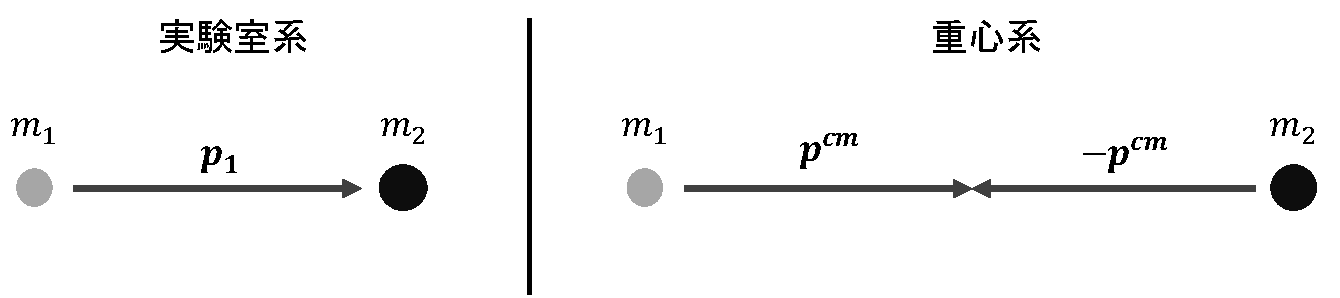
\includegraphics[width=12cm]{picture/relativity/initial.pdf}
\caption{始状態}
\label{fig:initial}
\end{figure}
\\
\\
\begin{figure}[htbp]
\centering
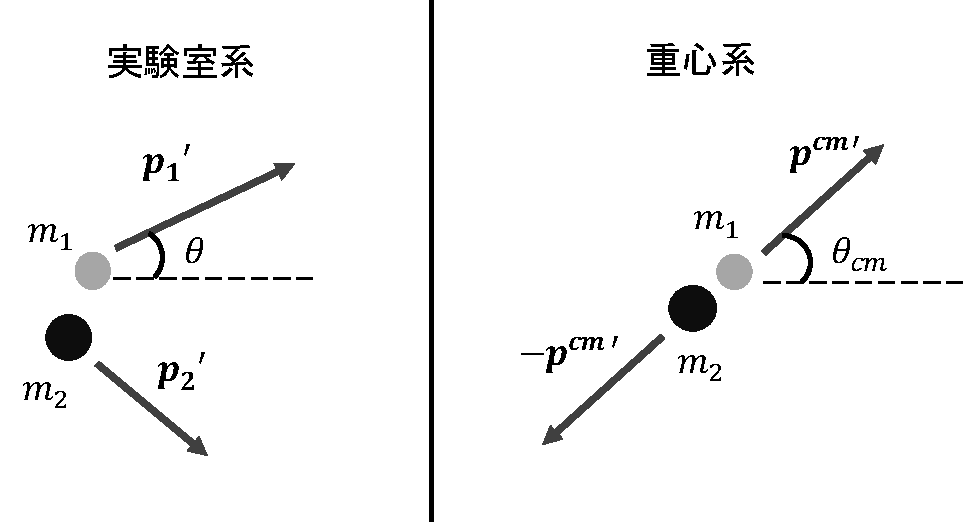
\includegraphics[width=9cm]{picture/relativity/final1.pdf}
\caption{終状態}
\label{fig:final}
\end{figure}
\newpage
\begin{equation}
    \left(
    \begin{array}{c}
     \frac{\varepsilon_{1}}{c}  \\
      p_{1}\\
      0 \\
      0
    \end{array}
  \right)  + \left(
    \begin{array}{c}
      m_{2}c \\
      0\\
      0 \\
      0
    \end{array}
  \right)=
      \left(
    \begin{array}{c}
     \frac{\varepsilon'_{1}}{c}  \\
      p'_{1x}\\
      p'_{1y}\\
      0
    \end{array}
  \right) +
    \left(
    \begin{array}{c}
     \frac{\varepsilon'_{2}}{c}  \\
      p'_{2x}\\
      p'_{2y}\\
      0
    \end{array}
  \right) \label{eq:yogen1}
\end{equation}
\begin{equation}
    \left(
    \begin{array}{c}
     \frac{\varepsilon_{1}^{cm}}{c}  \\
      p^{cm}\\
      0 \\
      0
    \end{array}
  \right)  + \left(
    \begin{array}{c}
      \frac{\varepsilon_{2}^{cm}}{c}  \\
      -p^{cm}\\
      0 \\
      0
    \end{array}
  \right)=
      \left(
    \begin{array}{c}
     \frac{\varepsilon^{cm'}_{1}}{c}  \\
      p^{cm'}_{x}\\
      p^{cm'}_{y}\\
      0
    \end{array}
  \right) +
    \left(
    \begin{array}{c}
     \frac{\varepsilon^{cm'}_{2}}{c}  \\
      -p^{cm'}_{x}\\
      -p^{cm'}_{y}\\
      0
    \end{array}
  \right) \label{eq:yogen2}
\end{equation}

また、この散乱は弾性散乱であり、
\begin{equation}
   s=\left(\frac{\varepsilon}{c}\right)^2-p^2=(mc)^2
\end{equation}
で表される$s$は散乱の前後で保存されるので、各粒子における$s$の保存より、
\begin{align}
     \left(\frac{\varepsilon'_{1}}{c}\right)^2-(\bm{p}'_{1})^2 = \left(\frac{\varepsilon^{cm}_{1}}{c}\right)^2-(\bm{p}^{cm})^2 =\left(\frac{\varepsilon^{cm'}_{1}}{c}\right)^2-(\bm{p}^{cm'})^2 \notag\\*
     =\left(\frac{\varepsilon_{1}}{c}\right)^2-(\bm{p}_{1})^2 = (m_{1}c)^2 \label{eq:snohozon}
\end{align}
\begin{equation}
    \left(\frac{\varepsilon'_{2}}{c}\right)^2-(\bm{p}'_{2})^2 = \left(\frac{\varepsilon^{cm}_{2}}{c}\right)^2-(\bm{p}^{cm})^2= 
     \left(\frac{\varepsilon^{cm'}_{2}}{c}\right)^2-(\bm{p}^{cm'})^2 =
     (m_{2}c)^2
\end{equation}

また、4元運動量の保存より
\begin{alignat}{3}
    \frac{\varepsilon^{cm}_{1}}{c} &= \frac{\varepsilon^{cm'}_{1}}{c}, &\qquad \frac{\varepsilon^{cm}_{2}}{c} &= \frac{\varepsilon^{cm'}_{2}}{c}, & \qquad 
    |\bm{p}^{cm}|&=|\bm{p}^{cm'}|
\end{alignat}
が言える。
次に、重心系での全エネルギーを$E^{cm}$とすると、始状態における全系のローレンツ不変量から、
\begin{equation*}
    \left(\frac{E^{cm}}{c}\right)^2 - 0 = \left(\frac{\varepsilon_{1}}{c} + m_{2}c\right)^{2} -(\bm{p_{1}})^2
\end{equation*}
\begin{equation}
   \therefore \left(\frac{E^{cm}}{c}\right)^2 = (m_{1}c)^{2} + (m_{2}c)^{2} + 2\frac{\varepsilon_{1}}{c}m_{2}c \qquad (\,\because\eqref{eq:snohozon})
\end{equation}

次にローレンツ変換のパラメータ$\beta$を求める。始状態の全系の変換は
\begin{equation}
    \left(
    \begin{array}{c}
     \frac{\varepsilon_{1}}{c} +m_{2}c \\
      p_{1}\\
      0 \\
      0
    \end{array}
  \right)  = \left(
    \begin{array}{cccc}
      \gamma & \beta\gamma & 0 & 0 \\
      \beta\gamma & \gamma & 0 & 0 \\
      0 & 0 & 1 & 0 \\
      0 & 0 & 0 & 1
    \end{array}
    \right) 
      \left(
    \begin{array}{c}
     \frac{E^{cm}}{c}  \\
      0\\
      0\\
      0
    \end{array}
  \right) =
    \left(
    \begin{array}{c}
     \gamma\frac{E^{cm}}{c}  \\
      \beta\gamma\frac{E^{cm}}{c}\\
      0\\
      0
    \end{array}
  \right) 
\end{equation}
\begin{equation}
    \therefore \gamma=\frac{\frac{\varepsilon_{1}}{c} +m_{2}c}{\frac{E^{cm}}{c}}
\end{equation}
また\;$\gamma=1/\sqrt{1-\beta^2}$より、
\begin{equation}
    \beta=\frac{\sqrt{\gamma^{2}-1}}{\gamma}=\frac{\sqrt{\left(\frac{\varepsilon_{1}}{c}\right)^2-(m_{1}c)^2}}{\frac{\varepsilon_{1}}{c} +m_{2}c}=\frac{p_{1}}{\frac{\varepsilon_{1}}{c} +m_{2}c}
\end{equation}
となる。
次に始状態、終状態それぞれにおける粒子1についての変換から、
\begin{equation}
    \left(
    \begin{array}{c}
     \frac{\varepsilon^{cm}_{1}}{c}  \\
      p^{cm}\\
      0 \\
      0
    \end{array}
  \right)  = \left(
    \begin{array}{cccc}
      \gamma & -\beta\gamma & 0 & 0 \\
      -\beta\gamma & \gamma & 0 & 0 \\
      0 & 0 & 1 & 0 \\
      0 & 0 & 0 & 1
    \end{array}
    \right) 
      \left(
    \begin{array}{c}
     \frac{\varepsilon_{1}}{c}  \\
      p_{1}\\
      0\\
      0
    \end{array}
  \right) =
    \left(
    \begin{array}{c}
     \gamma\left(\frac{\varepsilon_{1}}{c} -\beta p_{1}\right)  \\
      \gamma\left(p_{1}-\beta\frac{\varepsilon_{1}}{c}\right)\\
      0\\
      0
    \end{array}
  \right) 
\end{equation}
\begin{equation}
    \left(
    \begin{array}{c}
     \frac{\varepsilon'_{1}}{c}  \\
      p'_{1x}\\
      p'_{1y} \\
      0
    \end{array}
  \right)  = \left(
    \begin{array}{cccc}
      \gamma & \beta\gamma & 0 & 0 \\
      \beta\gamma & \gamma & 0 & 0 \\
      0 & 0 & 1 & 0 \\
      0 & 0 & 0 & 1
    \end{array}
    \right) 
      \left(
    \begin{array}{c}
     \frac{\varepsilon^{cm'}_{1}}{c}  \\
      p^{cm'}_{x}\\
      p^{cm'}_{y}\\
      0
    \end{array}
  \right) =
    \left(
    \begin{array}{c}
     \gamma\left(\frac{\varepsilon^{cm'}_{1}}{c} +\beta p^{cm'}_{x}\right)  \\
      \gamma\left(p^{cm'}_{x}+\beta\frac{\varepsilon^{cm'}_{1}}{c}\right)\\
      p^{cm'}_{y}\\
      0
    \end{array}
  \right) 
\end{equation}
よって、
\begin{align}
    \frac{p'_{1x}}{\gamma} &= p^{cm'}_{x}+ \beta\frac{\varepsilon^{cm'}_{1}}{c} = p^{cm'}_{x}+ \beta\frac{\varepsilon^{cm}_{1}}{c} \notag\\
    &= p^{cm'}_{x} + \beta\gamma\left(\frac{\varepsilon_{1}}{c}-\beta p_{1}\right) \notag\\
    &= p^{cm'}_{x} + \left[\frac{\frac{\varepsilon_{1}}{c}\left(\frac{\varepsilon_{1}}{c}+m_{2}c\right)}{\left(\frac{E^{cm}}{c}\right)^2}-\frac{\left(\frac{\varepsilon_{1}}{c}\right)^2-(m_{1}c)^2}{\left(\frac{E^{cm}}{c}\right)^2}\right]\frac{p_{1}}{\gamma} \notag\\
    &=  p^{cm'}_{x} +\frac{\frac{\varepsilon_{1}}{c}m_{2}c+(m_{1}c)^2}{\left(\frac{E^{cm}}{c}\right)^2}\frac{p_{1}}{\gamma} 
\end{align}
ここで、$x$成分のみを$\tfrac{1}{\gamma}$倍したベクトルを「$\;\Bar{}\;$」をつけて表すと、
\begin{alignat*}{2}
    \Bar{\bm{p}'_{1}} &= \left(\frac{p'_{1x}}{\gamma} \quad p'_{1y} \quad 0\right), &\quad  \Bar{\bm{p}_{1}} &= \left(\frac{p_{1x}}{\gamma} \quad 0 \quad 0\right) 
\end{alignat*}
であり、
\begin{equation}
     \Bar{\bm{p}'_{1}} = \bm{p}^{cm'} +\frac{\frac{\varepsilon_{1}}{c}m_{2}c+(m_{1}c)^2}{\left(\frac{E^{cm}}{c}\right)^2}\Bar{\bm{p}_{1}}\label{eq:p1}
\end{equation}
が成り立つ。粒子2についても同様に、
\begin{equation}
    \left(
    \begin{array}{c}
     \frac{\varepsilon^{cm}_{2}}{c}  \\
      -p^{cm}\\
      0 \\
      0
    \end{array}
  \right)  = \left(
    \begin{array}{cccc}
      \gamma & -\beta\gamma & 0 & 0 \\
      -\beta\gamma & \gamma & 0 & 0 \\
      0 & 0 & 1 & 0 \\
      0 & 0 & 0 & 1
    \end{array}
    \right) 
      \left(
    \begin{array}{c}
     m_{2}c\\
      0\\
      0\\
      0
    \end{array}
  \right) =
    \left(
    \begin{array}{c}
     \gamma m_{2}c\\
      -\beta\gamma m_{2}c\\
      0\\
      0
    \end{array}
  \right) 
\end{equation}
\begin{equation}
    \left(
    \begin{array}{c}
     \frac{\varepsilon'_{2}}{c}  \\
      p'_{2x}\\
      p'_{2y} \\
      0
    \end{array}
  \right)  = \left(
    \begin{array}{cccc}
      \gamma & \beta\gamma & 0 & 0 \\
      \beta\gamma & \gamma & 0 & 0 \\
      0 & 0 & 1 & 0 \\
      0 & 0 & 0 & 1
    \end{array}
    \right) 
      \left(
    \begin{array}{c}
     \frac{\varepsilon^{cm'}_{2}}{c}  \\
      -p^{cm'}_{x}\\
      -p^{cm'}_{y}\\
      0
    \end{array}
  \right) =
    \left(
    \begin{array}{c}
     \gamma\left(\frac{\varepsilon^{cm'}_{2}}{c} -\beta p^{cm'}_{x}\right)  \\
      \gamma\left(-p^{cm'}_{x}+\beta\frac{\varepsilon^{cm'}_{2}}{c}\right)\\
      -p^{cm'}_{y}\\
      0
    \end{array}
  \right) 
\end{equation}
より
\begin{align}
    \frac{p'_{2x}}{\gamma} &= -p^{cm'}_{x}+ \beta\frac{\varepsilon^{cm'}_{2}}{c} = -p^{cm'}_{x}+ \beta\frac{\varepsilon^{cm}_{2}}{c} \notag\\
    &= -p^{cm'}_{x} + \beta\gamma m_{2}c \notag\\
    &= -p^{cm'}_{x} +\frac{\left(\frac{\varepsilon_{1}}{c}+m_{2}c\right)m_{2}c}{\left(\frac{E^{cm}}{c}\right)^2}\frac{p_{1}}{\gamma} 
\end{align}
だから、
\begin{equation*}
    \Bar{\bm{p}'_{2}} = \left(\frac{p'_{2x}}{\gamma} \quad p'_{2y} \quad 0\right)
\end{equation*}
として
\begin{equation}
     \Bar{\bm{p}'_{2}} = -\bm{p}^{cm'} +\frac{\left(\frac{\varepsilon_{1}}{c}+m_{2}c\right)m_{2}c}{\left(\frac{E^{cm}}{c}\right)^2}\Bar{\bm{p}_{1}}\label{eq:p2}
\end{equation}
となる。

ここで、 $\Bar{\bm{p}_{1}}$と$\Bar{\bm{p}'_{1}}$ のなす角を$\Bar{\theta}$とすると、
\begin{equation}
    \tan\Bar{\theta}=\frac{p'_{1y}}{p'_{1x}/\gamma}=\gamma\tan\theta \label{eq:bartheta}
\end{equation}
また、$n=\left(\frac{\varepsilon_{1}}{c}m_{2}c + (m_{2}c)^2\right)/\left(\frac{\varepsilon_{1}}{c}m_{2}c + (m_{1}c)^2\right)$とすれば以前の結果を用いて、
\begin{equation}
    \tan\Bar{\theta} = \frac{\sin\theta_{cm}}{\cos\theta_{cm}+\frac{1}{n}} \label{eq:barcm}
\end{equation}
となる。
よって、式\eqref{eq:bartheta}と\eqref{eq:barcm}より
\begin{equation}
    \tan\theta = \frac{\sin\theta_{cm}}{\gamma\left(\cos\theta_{cm}+\frac{1}{n}\right)} \label{eq:henkan3}
\end{equation}
これが相対論における実験室系での散乱角$\theta$と重心系での散乱角$\theta_{cm}$を関係づける式である。

例えばp-p散乱の場合、$m_{1}=m_{2}$より$n=1$となり、式\eqref{eq:barcm}から
\begin{equation}
    \Bar{\theta}=\frac{\theta_{cm}}{2}
\end{equation}
となる。よって、
\begin{equation}
    \theta=\arctan\left(\frac{\tan\frac{\theta_{cm}}{2}}{\gamma}\right)
\end{equation}
となる。

また、実験室系と重心系における微分散乱断面積をそれぞれ$\left(\frac{d\sigma}{d\Omega}\right)_\text{lab}$,$\left(\frac{d\sigma}{d\Omega}\right)_\text{cm}$とすると、これらの間の関係式は、相対論の効果を考慮すると
\begin{equation}
    \left(\frac{d\sigma}{d\Omega}\right)_\text{cm} = \frac{\gamma\left(1+\frac{\cos\theta_{cm}}{n}\right)}{\left(\sin^2\theta_{cm}+\gamma^2\left(\cos\theta_{cm}+\frac{1}{n}\right)^2\right)^{\frac{3}{2}}}\left(\frac{d\sigma}{d\Omega}\right)_\text{lab}\label{eq:henkan4}
\end{equation}
と書ける。

以上から、相対論を考慮する場合は非相対論の変換式\eqref{eq:henkan1},\eqref{eq:henkan2}はそれぞれ\eqref{eq:henkan3},\eqref{eq:henkan4}に変化することがわかる。

\end{document}